%!TEX root=paper.tex

\newpage
\section{What is the Perception of the Learners?}
\label{sec:perception}

\subsection{About The Reader}

After the semester was over, we sent an email asking the students to answer the survey about their experience and received \surveyrespondents answers. Figure \ref{fig:reader_use} summarizes the answers to the first question that asked the respondents to rate the ease of use (top) and usefulness (bottom) of the reader. 

 \begin{figure}[h!]
    \centering
      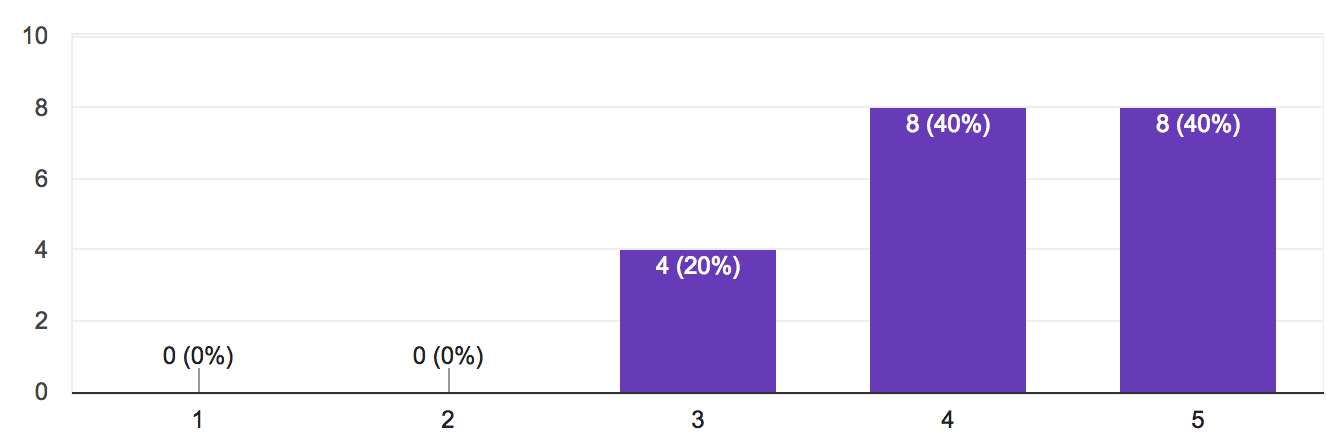
\includegraphics[width=0.8\columnwidth]{figures/opinions/reader_ease_of_use}
      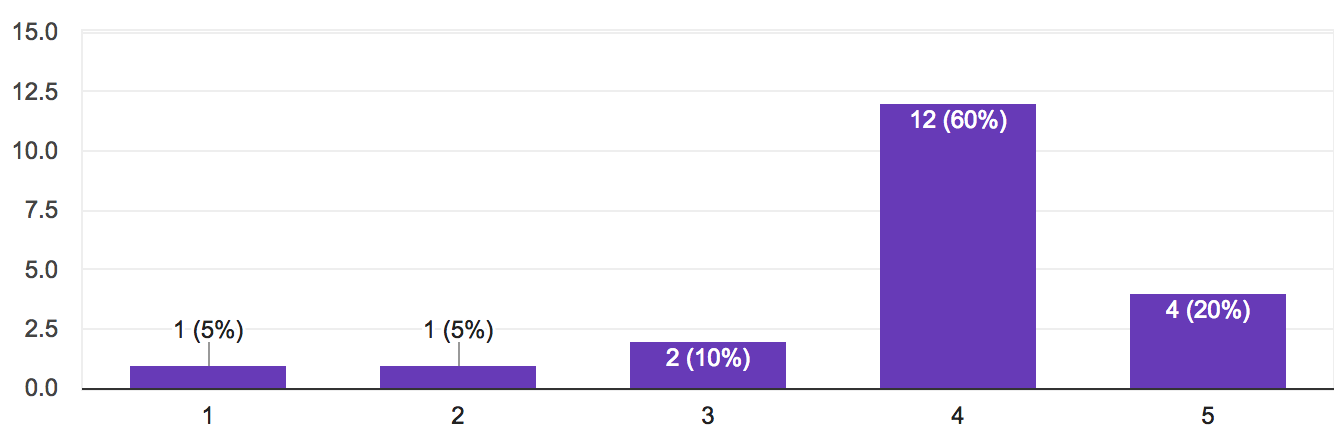
\includegraphics[width=0.8\columnwidth]{figures/opinions/reader_usefulness}
      \caption{Feedback on Reader ease of use (top) and usefulness (bottom)}
      \label{fig:reader_use}
    \end{figure}

When asked what would make their experience with the Reader better many of the students thought that the system was good the way it was and few had some very specific features in mind (e.g. night reading mode\footnote{Complete feedback available in the GitHub repository of the paper.}). There was however, one request which was expressed multiple times, even if in slightly diffferent ways by multiple respondents: the need for more specificity in the selection of materials to read. The students suggested: \squote{Order articles in different subjects like Animals, Politics, Fashion...},\squote{Better display of the articles and tags such as Gaming or News}, \squote{Add a choice for different topics not only for the sources}, \squote{Add a search engine}. 

    % \item \squote{Be able to add website to the list} and \squote{Add a search engine}
% \end{itemize}

When asked about what they dislike about the Reader, the majority of feedback was related to translations: two people complained about them being in English (\squote{The translations are always in English}), five people complained about the translation quality (e.g. \squote{Some weak translations}). The English translations are the reason for which one learner reported that they prefer the textbook: \squote{The translations are always in English. This is why I would grab a textbook first. I don't want to look up the (English to) Dutch translation.}


We also asked students how would they prefer reading texts in their foreign language.
 % We thus asked them what would they choose between the our system (Zeeguu Reader in the figure) and a textbook. 
 % We also gave them the possibility to answer something else with a free-form text field. 
 Figure \ref{fig:preferred_reader} shows that the majority of the learners who answered our post-usage survey would prefer our system (Zeeguu Reader). However, some still prefer a textbook, probably for the reasons enumerated above.

 \begin{figure}[h!]
    \centering
      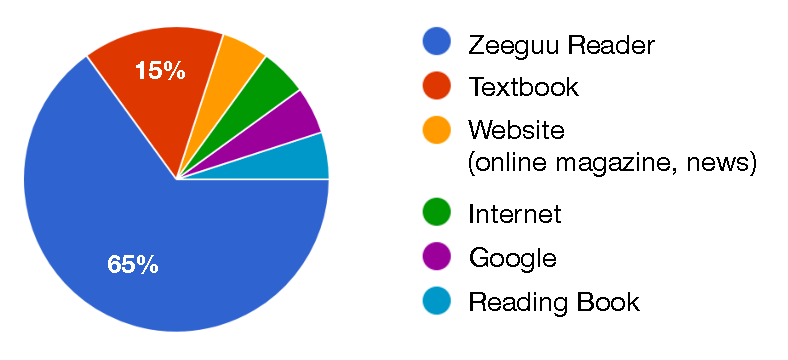
\includegraphics[width=0.6\columnwidth]{figures/opinions/reader_vs_textbook.pdf}
      \caption{Answers to the question: {``If you wanted to read something in the language you study, what would you reach out for first?''}}
      \label{fig:preferred_reader}
    \end{figure}



\subsection{About The Exercises}
Figure \ref{fig:ex_rating} shows that when asked to provide their personal rating of the the quality of the exercises, the majority of the respondents are positive: 

 \begin{figure}[h!]
    \centering
      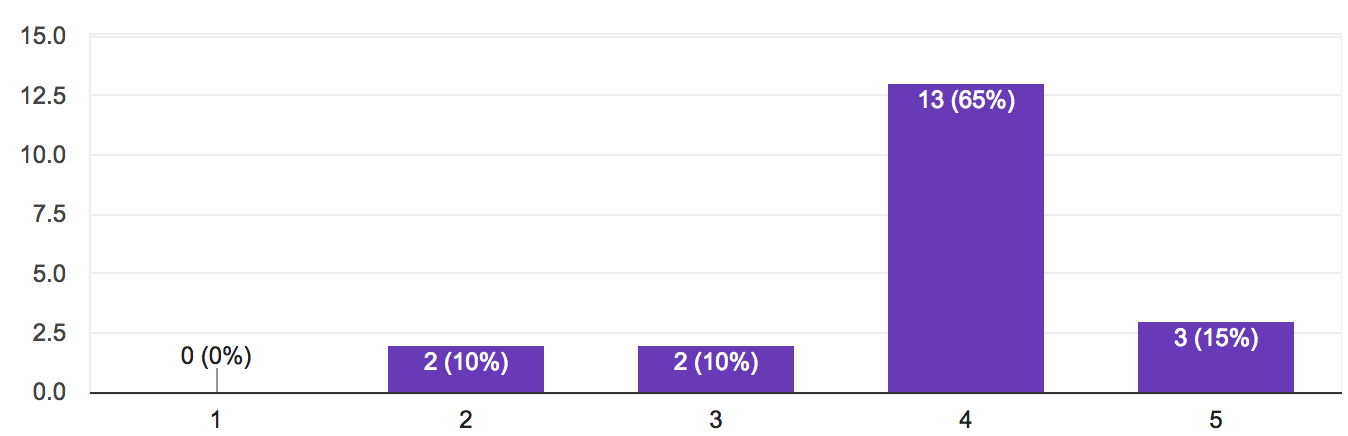
\includegraphics[width=0.8\columnwidth]{figures/opinions/exercises_rating}
      \caption{Students assessment  of the generated exercises}
      \label{fig:ex_rating}
    \end{figure}

When asked about what they dislike about exercises, many said literally ``nothing''. However, several also had concrete feedback that can be classified in two main directions: 

\begin{enumerate}

  \item Contexts are always the same: \squote{I would like to see the words I practice in a different context}. This would indeed be an idea worthy of further investigation.

	\item Exercises can be too easy. One learner wrote in their feedback that \squote{some exercises are too easy}. 

  \item Exercises can be too difficult. Some learners encountered exercises in which they did not understand well the context, and would have wanted translations for it. However, translations are not enabled during exercises, so they reported that: \squote{There aren't translations}, \squote{Doesn't give the translations}. 
	
\end{enumerate}

\subsection{About The Overall System}
% During the running of the experiment, randomly selected students were asked a series of questions by popping up questions while they were using the system. For this, we used an online tool called HotJar. Among the questions was whether they preferred the reading platform and why. Some of the answers can be seen in the screenshot below. It becomes clear that the students appreciate the possibility of reading what is interesting for them.

%     \begin{figure}[h!]
%     \centering
%       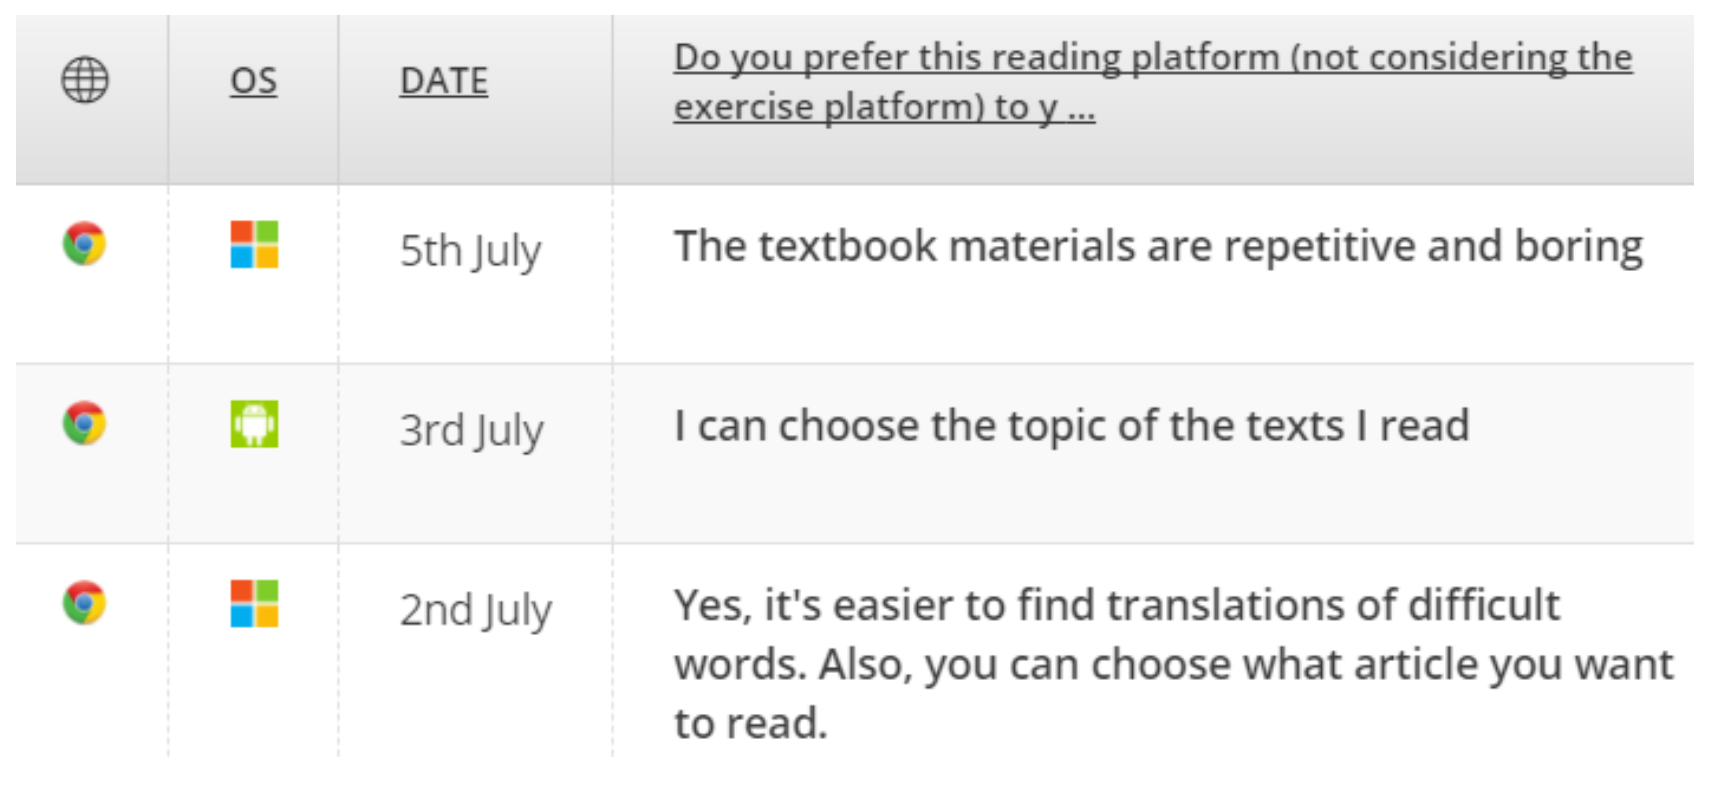
\includegraphics[width=0.7\columnwidth]{figures/opinion_on_reading_platform}
%       \caption{The students appreciate the freedom of choosing what to read}
%     \end{figure}


% \newpage
% \subsection{Reports to the Teacher}
At the end of the semester, the students had to provide feedback to their teacher about all of the software tools they used in the class during the year. This is something that the teacher always does at the end of the school year. Since the students had to write also about our system, we asked the teacher if we could access the corresponding feedback and they were glad to oblige. 

Six students wrote more detailed opinions. The main ideas in the feedback are illustrated by the three example quotes listed below\footnote{Although the original feedback is in Dutch, we translated all the  detailed answers and uploaded them online in the associated data repository of the paper as {\em feedback-to-the-teacher.txt}}: 

\begin{description}
  \item {\em ``It's good for improving reading skills. It would be even better if this tool was available in Dutch''}
  \item {\em ``Works well, but if it were possible to translate to Dutch it would have been better. Good that you can choose what you read.''}
  \item {\em ``My vocabulary truly is improving, but you do have to use it more than a few times. A very nice website, easy to use and with nice topics''}
\end{description}


Thus, learners appreciate the freedom of choosing materials to read that are personally interesting for them. They also appreciate the translations, but they would want to have them in their native language. 


% The way forward is then, by providing better recommendations if possible, and by providing translations in their native languages.

% In the future we plan to investigate whether the system works well enough with Dutch.
